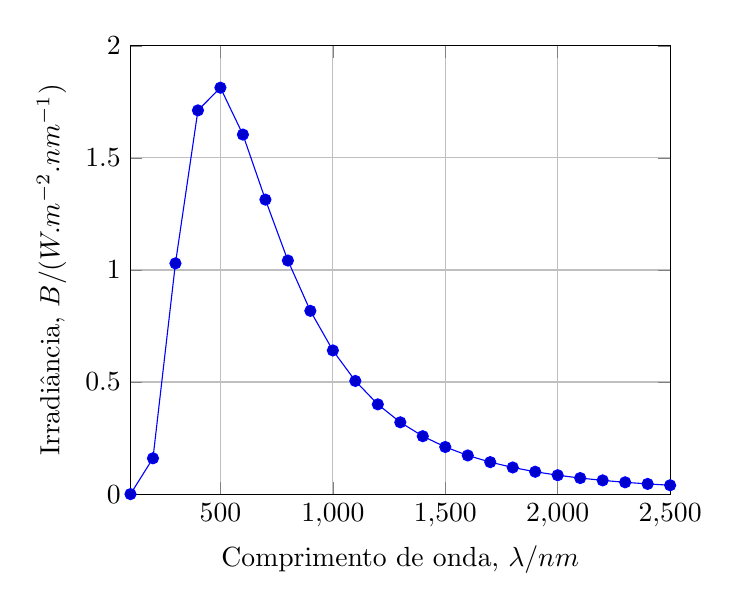
\begin{tikzpicture}
    \def\kB{1.4e-23}
    \def\hc{6.6*3e-17}
    \begin{axis}
        [
            grid = both,
            xlabel={Comprimento de onda, $\lambda/\si{nm}$},
            ylabel={Irradiância, $B/(\si{W.m^{-2}.nm^{-1}})$},
            domain=100:2500,
            xmin=100, ymin=0,
            xmax=2500, ymax=2,
        ]
    \pgfplotsinvokeforeach{6000}
        {
            \addplot
            {
                2*3.14*6.6*9*1.6e13/(x^5*(exp(1.4e7/(#1*x))-1))
            };
        }
    \end{axis}
\end{tikzpicture}